\documentclass[tikz,border=10pt]{standalone}
\usetikzlibrary{shapes.geometric, arrows.meta}

\tikzset{
    block/.style = {rectangle, draw, text width=5em, text centered, rounded corners, minimum height=4em},
    line/.style = {draw, thick, -Stealth}
}

\begin{document}

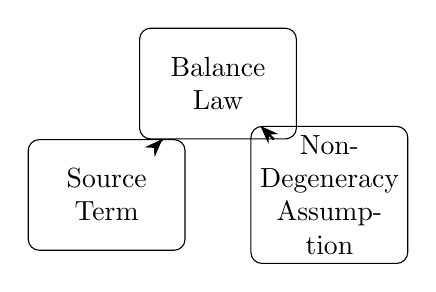
\begin{tikzpicture}[node distance=2cm]

\node (balanceLaw) [block] {Balance Law};
\node (sourceTerm) [block, below left of=balanceLaw] {Source Term};
\node (nonDegeneracyAssumption) [block, below right of=balanceLaw] {Non-Degeneracy Assumption};

% Drawing lines between nodes
\draw [line] (balanceLaw) -- (sourceTerm);
\draw [line] (balanceLaw) -- (nonDegeneracyAssumption);

\end{tikzpicture}

\end{document}